
\begin{sidewaysfigure}
    \centering    
    \caption{Empirical example: Comparison of group-level emission distribution means and variances estimates for the MEDHMM and MHMM}
 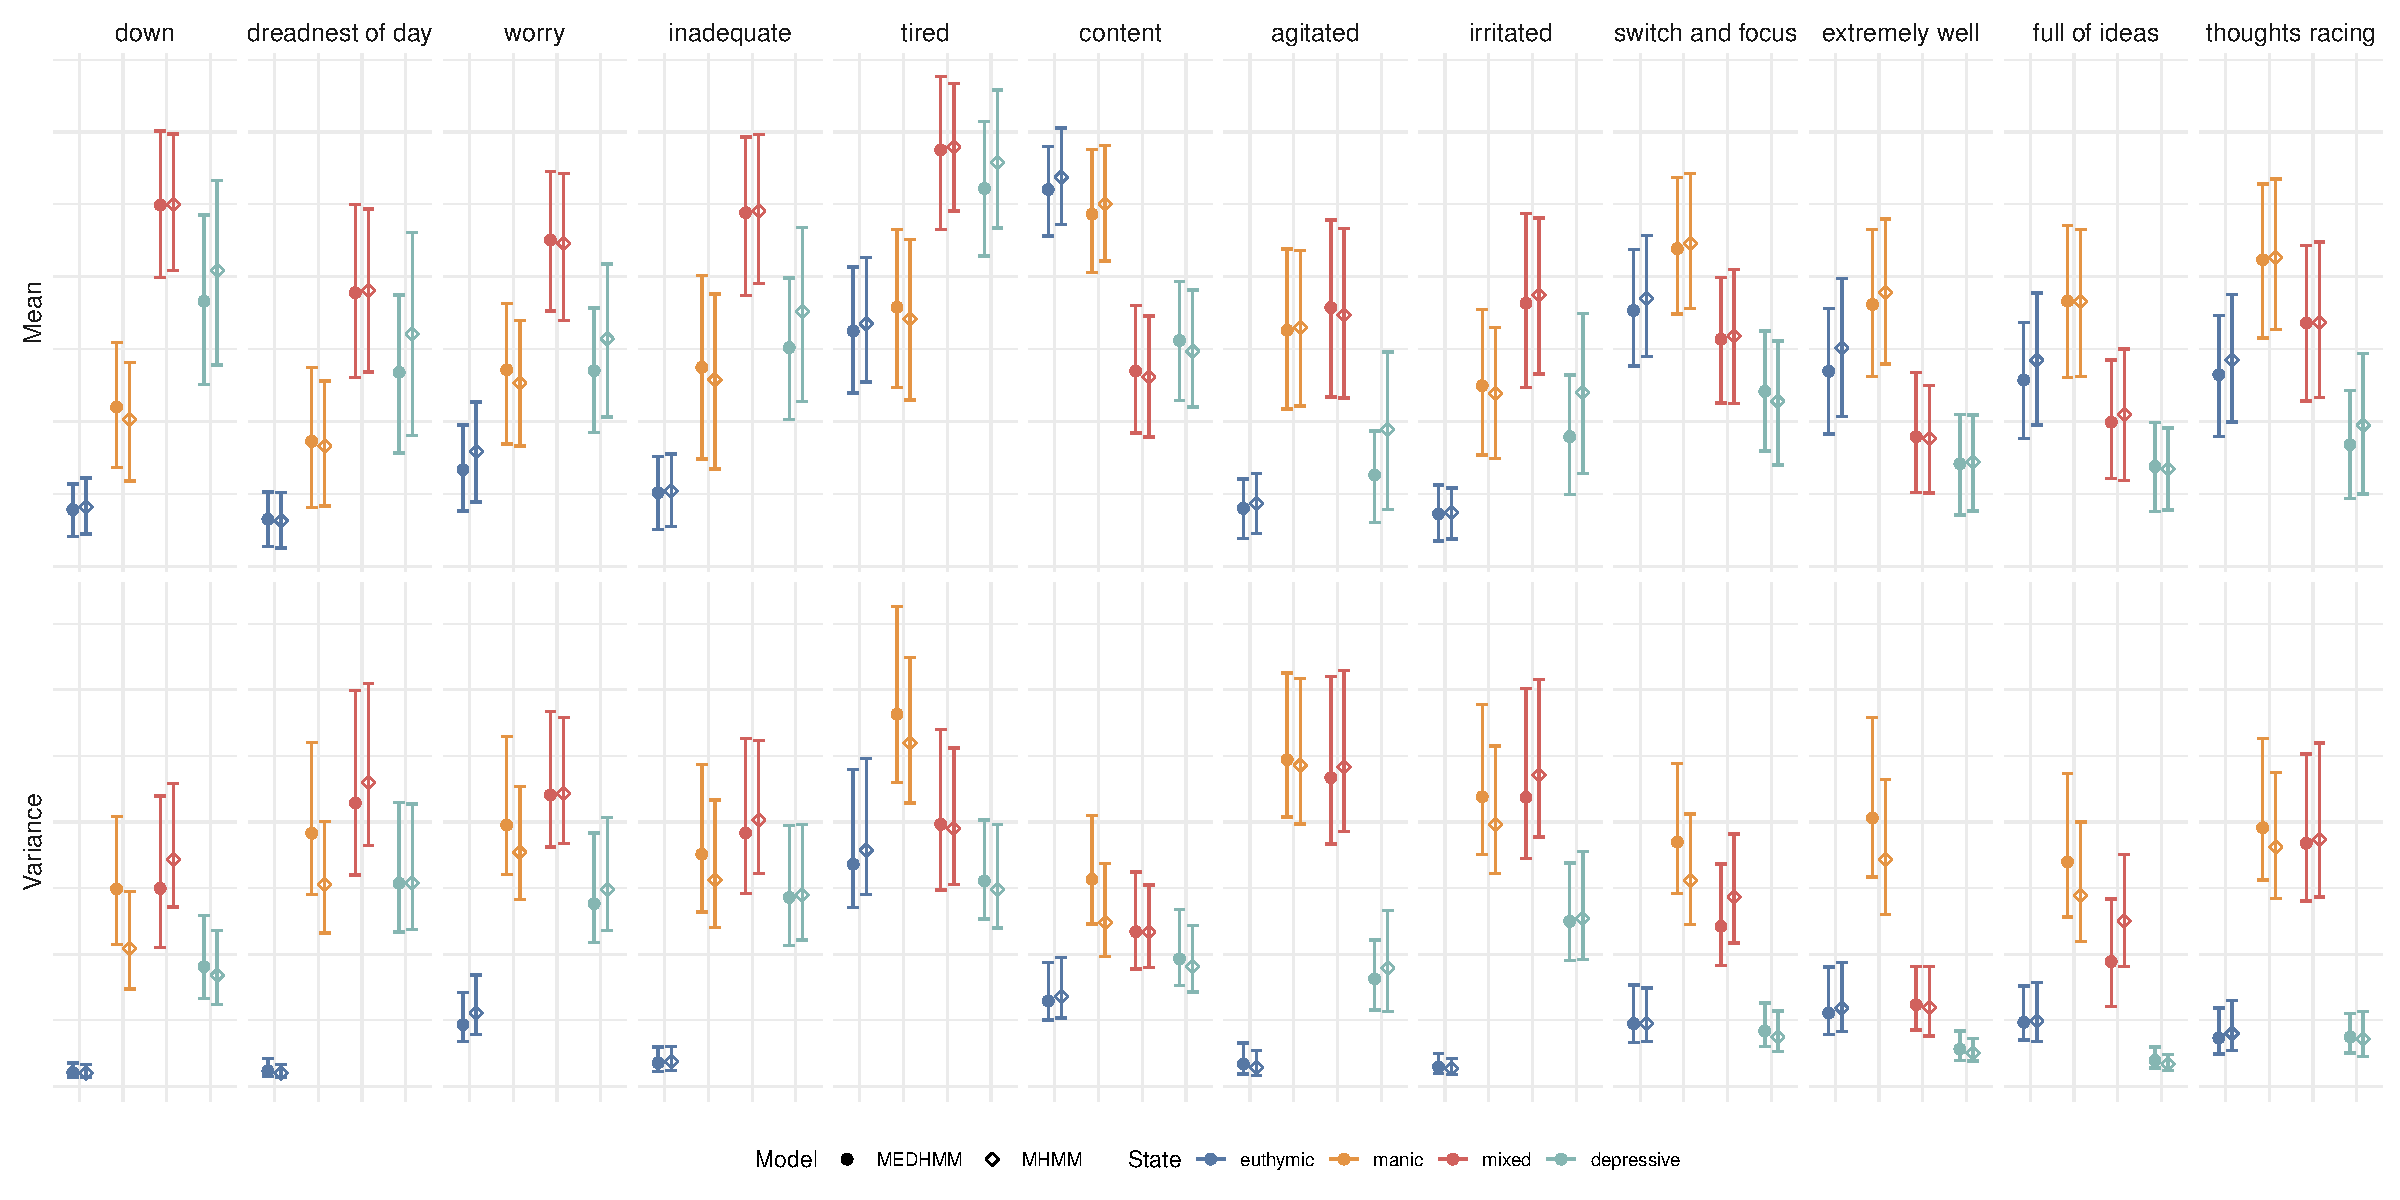
\includegraphics[scale=0.6]{graphics/comparison_emiss_group_level2.pdf}
 \flushleft
 \footnotesize
 \justifying
 This figure shows comparison between group-level estimates of emission distribution parameters. The first row contains estimates for emission means, and the second row shows the emission variances. Each vertical panel represents a dependent variable (inspected EMA item). Within each plot for dependent variable parameters, each Bipolar disorder mood state-specific estimate is marked with a different colour. The round points are indicators of MHMM and diamond points are the MEDHMM estimates. 
    \label{group_emission_emp}
\end{sidewaysfigure}

\begin{figure}
    \centering    
    \caption{Empirical example: Temporal alignment between mood states and weekly symptom scores}
 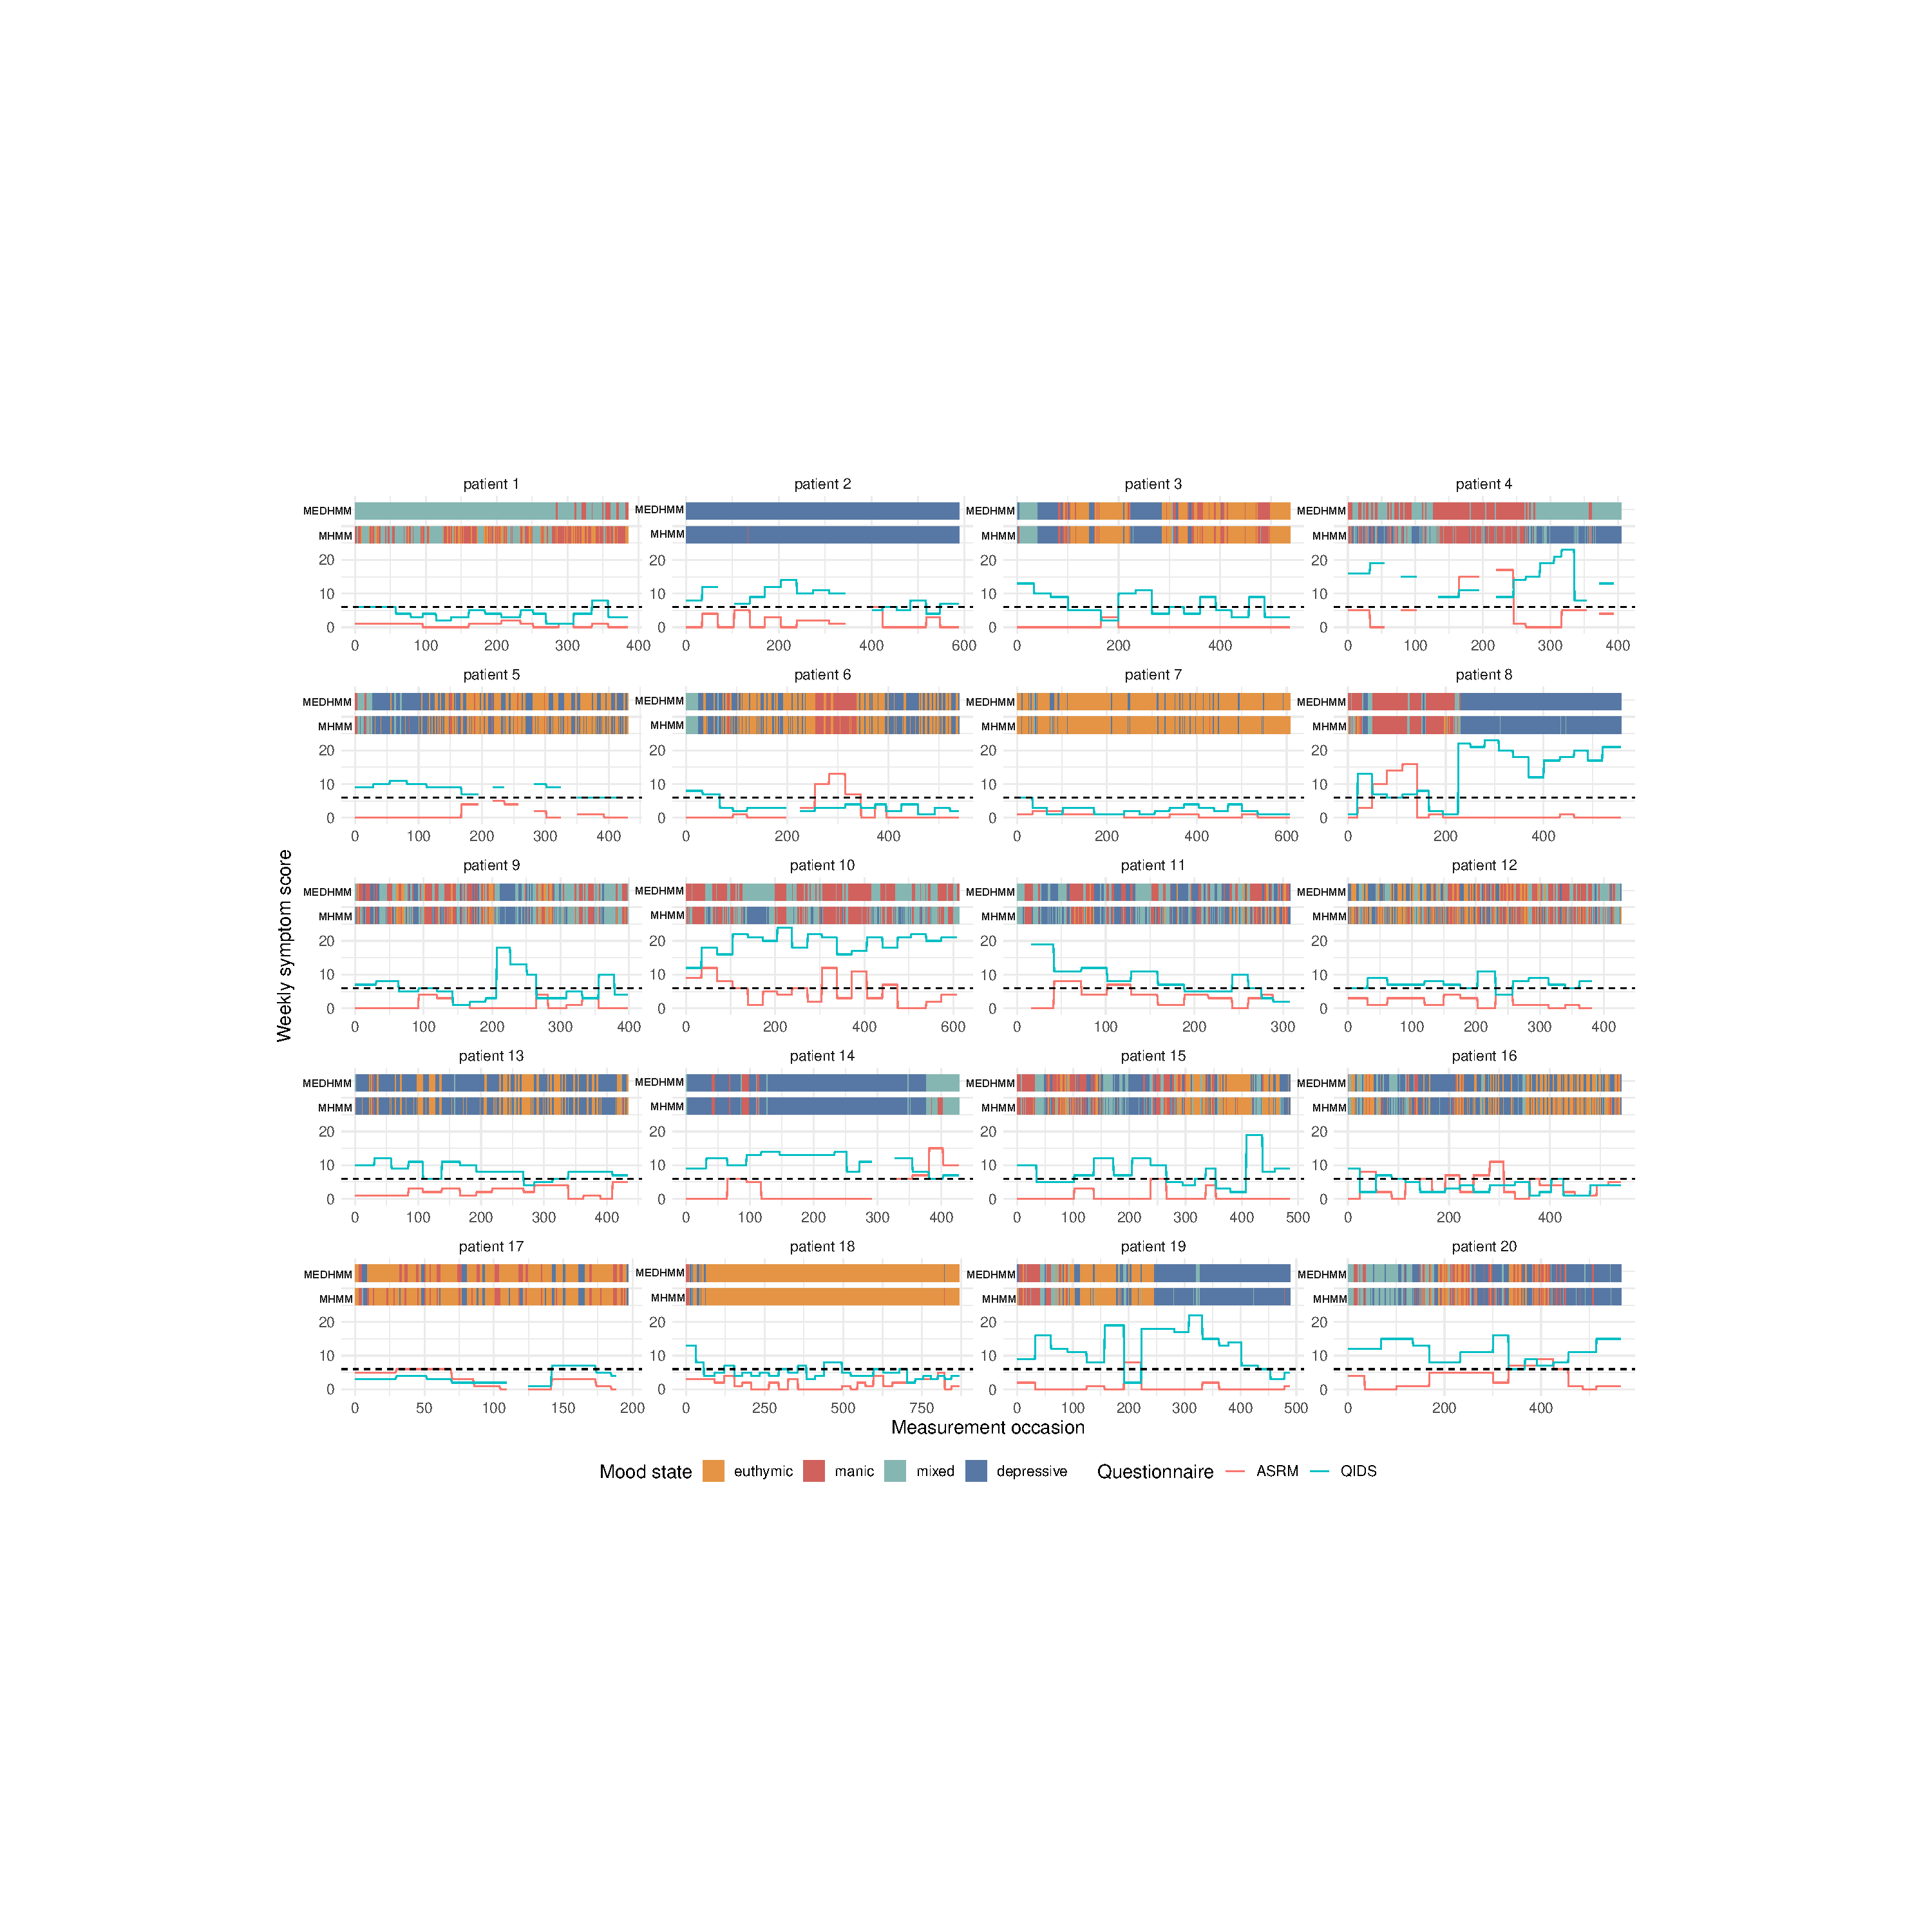
\includegraphics[width=\linewidth]{graphics/decoding_all.pdf}
 \flushleft
 \footnotesize
 The figure shows local state decodings for the MEDHMM (upper decoding strip) and the MHMM (lower decoding script). The plots are presented for all Bipolar disorder patients. Under the strip plots the alignment with the weekly symptom scores on depressive behaviour indicator (QIDS) and manic behaviour indicator (ASRM).
    \label{decoding_all}
\end{figure}

% Please add the following required packages to your document preamble:
% \usepackage{booktabs}
% \usepackage{lscape}

\begin{table}[h]
\caption{Empirical example: Analysis of switches between states \& empirically assessed average state durations}
\resizebox{\linewidth}{!}{
\begin{tabular}{cccccccc}
  \toprule
   &  & \multicolumn{6}{c}{MEDHMM}\\ \cmidrule{3-8}
\textbf{Patient no.} &
 \textbf{Observations} &
 \textbf{Switches count} &
  \textbf{Relative proportion of switches} &
  \textbf{Euthymic state} &
  \textbf{Manic state} &
  \textbf{Mixed state} &
  \textbf{Depressive state}  \\ \midrule

1 & 386 & 16 & 0.041 & 4.83 & 5.71 & 6.69 & 5.10 \\
2 & 589 & 0 & 0 & 4.79 & 4.29 & 4.41 & 5.07 \\
3 & 538 & 61 & 0.113 & 6.84 & 3.27 & 4.82 & 7.10 \\
4 & 405 & 41 & 0.101 & 4.91 & 4.82 & 4.23 & 5.15 \\
5 & 431 & 71 & 0.165 & 5.03 & 2.94 & 4.74 & 4.81 \\
6 & 540 & 83 & 0.154 & 4.92 & 8.18 & 5.20 & 4.13 \\
7 & 608 & 47 & 0.077 & 13.32 & 4.30 & 4.08 & 2.91 \\
8 & 559 & 16 & 0.029 & 4.31 & 11.25 & 4.43 & 8.36 \\
9 & 399 & 99 & 0.248 & 3.41 & 3.42 & 4.03 & 3.41 \\
10 & 613 & 50 & 0.082 & 4.78 & 7.68 & 5.81 & 5.04 \\
11 & 308 & 84 & 0.273 & 2.75 & 3.85 & 3.96 & 4.14 \\
12 & 427 & 115 & 0.269 & 2.99 & 3.80 & 3.69 & 3.43 \\
13 & 434 & 60 & 0.138 & 3.92 & 3.60 & 4.11 & 6.45 \\
14 & 428 & 16 & 0.037 & 4.83 & 5.14 & 3.59 & 17.90 \\
15 & 486 & 95 & 0.195 & 4.28 & 3.87 & 3.83 & 3.63 \\
16 & 541 & 111 & 0.205 & 3.60 & 3.58 & 4.00 & 4.57 \\
17 & 197 & 44 & 0.223 & 5.20 & 2.67 & 4.24 & 3.13 \\
18 & 869 & 13 & 0.015 & 11.89 & 4.84 & 4.07 & 4.27 \\
19 & 489 & 40 & 0.082 & 5.56 & 5.15 & 4.03 & 6.26 \\
20 & 566 & 95 & 0.168 & 3.41 & 3.42 & 4.59 & 5.91 \\
\bottomrule
\end{tabular}}


\resizebox{\linewidth}{!}{
\begin{tabular}{cccccccc}
  \toprule
   & &  \multicolumn{6}{c}{MHMM}\\ \cmidrule{3-8}
\textbf{Patient no.} &
 \textbf{Observations} &
  \textbf{Switches count} &
  \textbf{Relative proportion of switches} &
  \textbf{Euthymic state} &
  \textbf{Manic state} &
 \textbf{Mixed state} &
  \textbf{Depressive state} \\ \midrule
1 & 386 & 141 & 0.365 & 2.66 & 6.29 & 9.52 & 3.50 \\
2 & 589 & 2 & 0.003 & 2.98 & 2.85 & 2.97 & 254.56 \\
3 & 538 & 72 & 0.134 & 26.31 & 5.51 & 12.60 & 21.61 \\
4 & 405 & 137 & 0.338 & 3.09 & 8.45 & 3.54 & 11.39 \\
5 & 431 & 151 & 0.35 & 6.93 & 2.60 & 5.07 & 6.36 \\
6 & 540 & 147 & 0.272 & 8.68 & 14.41 & 11.73 & 5.44 \\
7 & 608 & 74 & 0.122 & 41.29 & 2.57 & 2.92 & 2.35 \\
8 & 559 & 58 & 0.104 & 2.51 & 20.07 & 5.88 & 43.41 \\
9 & 399 & 170 & 0.426 & 3.73 & 4.95 & 6.13 & 4.96 \\
10 & 613 & 157 & 0.256 & 3.12 & 13.04 & 7.04 & 7.17 \\
11 & 308 & 172 & 0.558 & 1.84 & 4.21 & 3.97 & 4.69 \\
12 & 427 & 252 & 0.59 & 3.30 & 3.38 & 3.48 & 2.66 \\
13 & 434 & 117 & 0.27 & 6.06 & 2.85 & 2.98 & 9.47 \\
14 & 428 & 24 & 0.056 & 3.19 & 9.10 & 10.87 & 74.51 \\
15 & 486 & 192 & 0.395 & 7.13 & 5.14 & 5.47 & 4.86 \\
16 & 541 & 225 & 0.416 & 5.77 & 3.01 & 4.04 & 5.94 \\
17 & 197 & 68 & 0.345 & 9.54 & 2.05 & 3.23 & 3.87 \\
18 & 869 & 23 & 0.026 & 172.36 & 4.53 & 2.99 & 5.41 \\
19 & 489 & 70 & 0.143 & 14.20 & 8.53 & 4.86 & 30.46 \\
20 & 566 & 181 & 0.32 & 5.72 & 4.75 & 8.38 & 10.01 \\

\bottomrule
\end{tabular}}

\label{table_emp_switch}
\end{table}